\documentclass[compress]{beamer}
\usepackage{ifthen,verbatim}

\setbeamertemplate{navigation symbols}{}

\begin{document}

\begin{frame}
\frametitle{How many QCD muons with a given $p_T$ cut?}
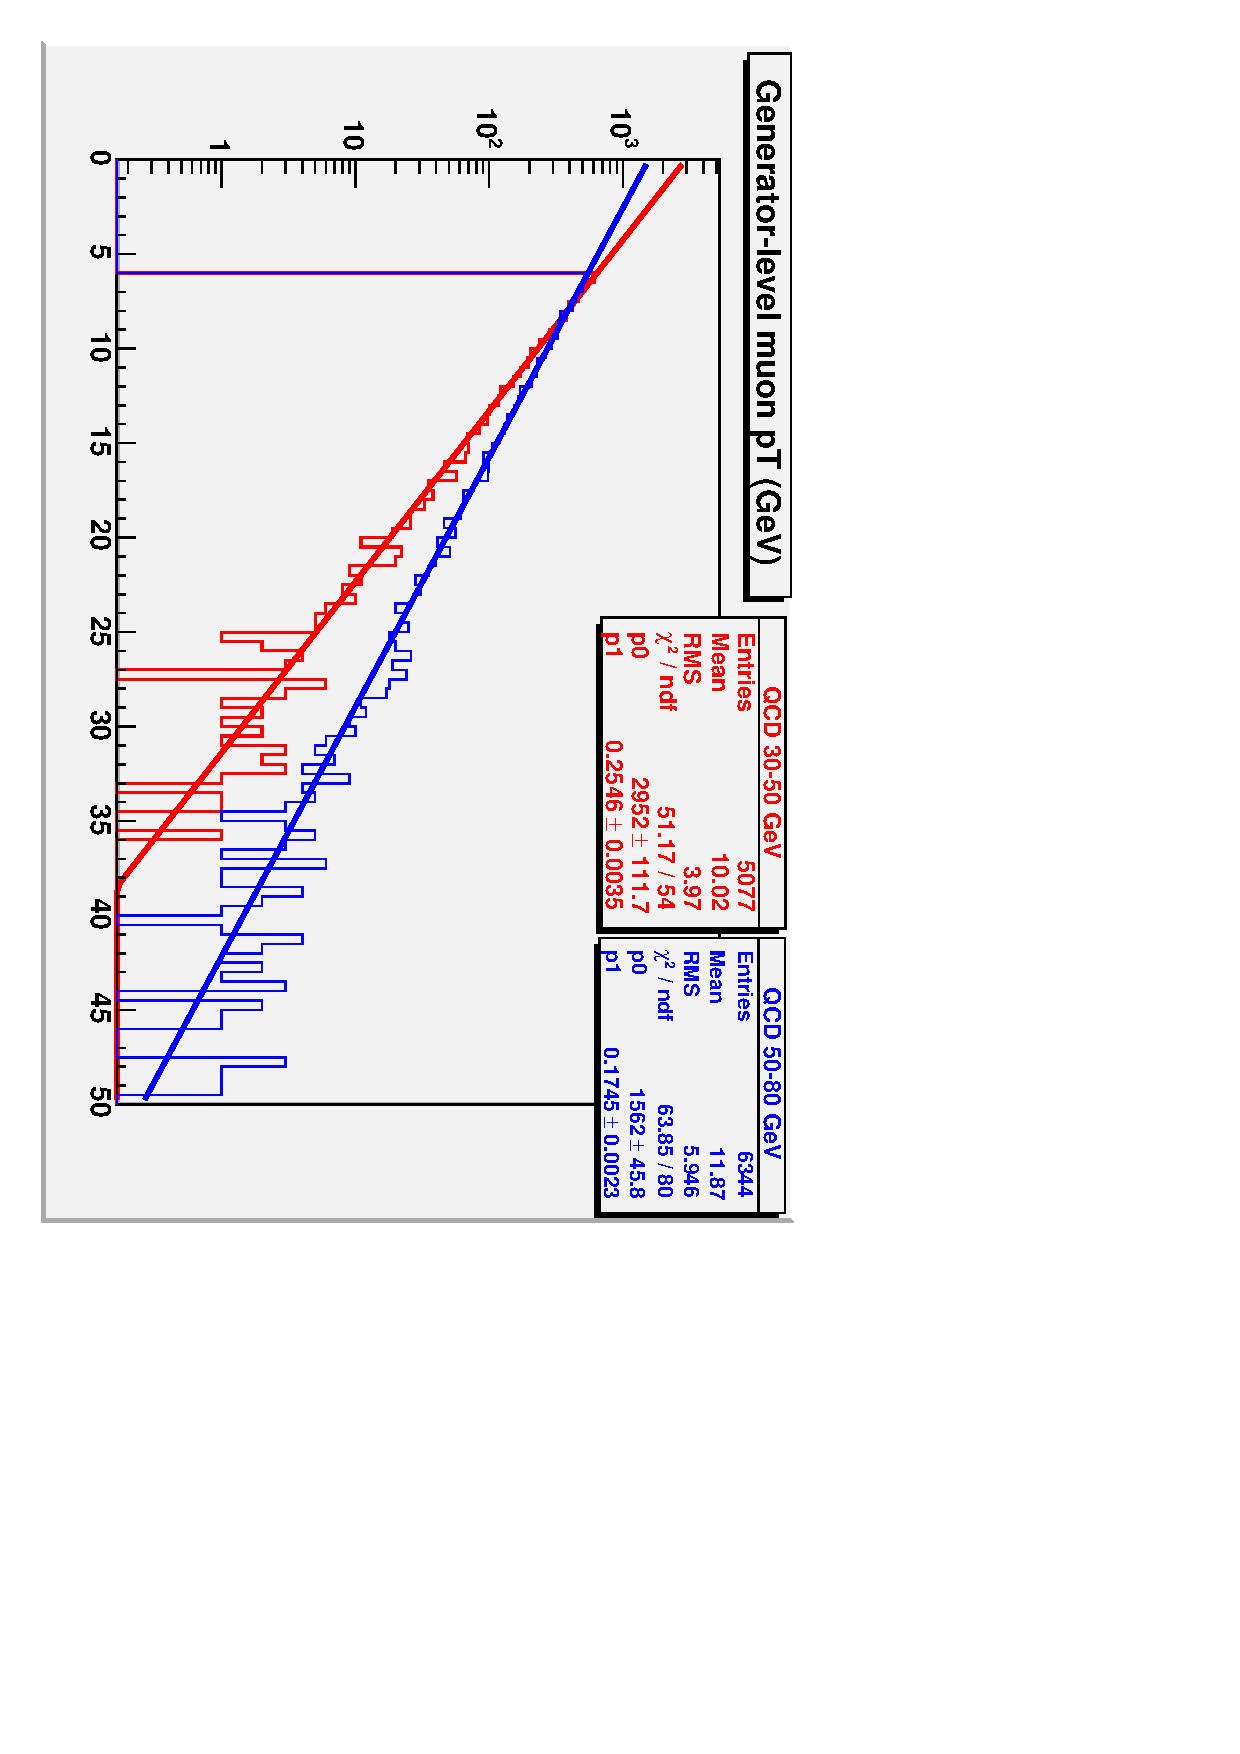
\includegraphics[height=\linewidth, angle=90]{exponential_qcd.pdf}
\end{frame}

\begin{frame}
\frametitle{Spectrum for ``physics muons''}
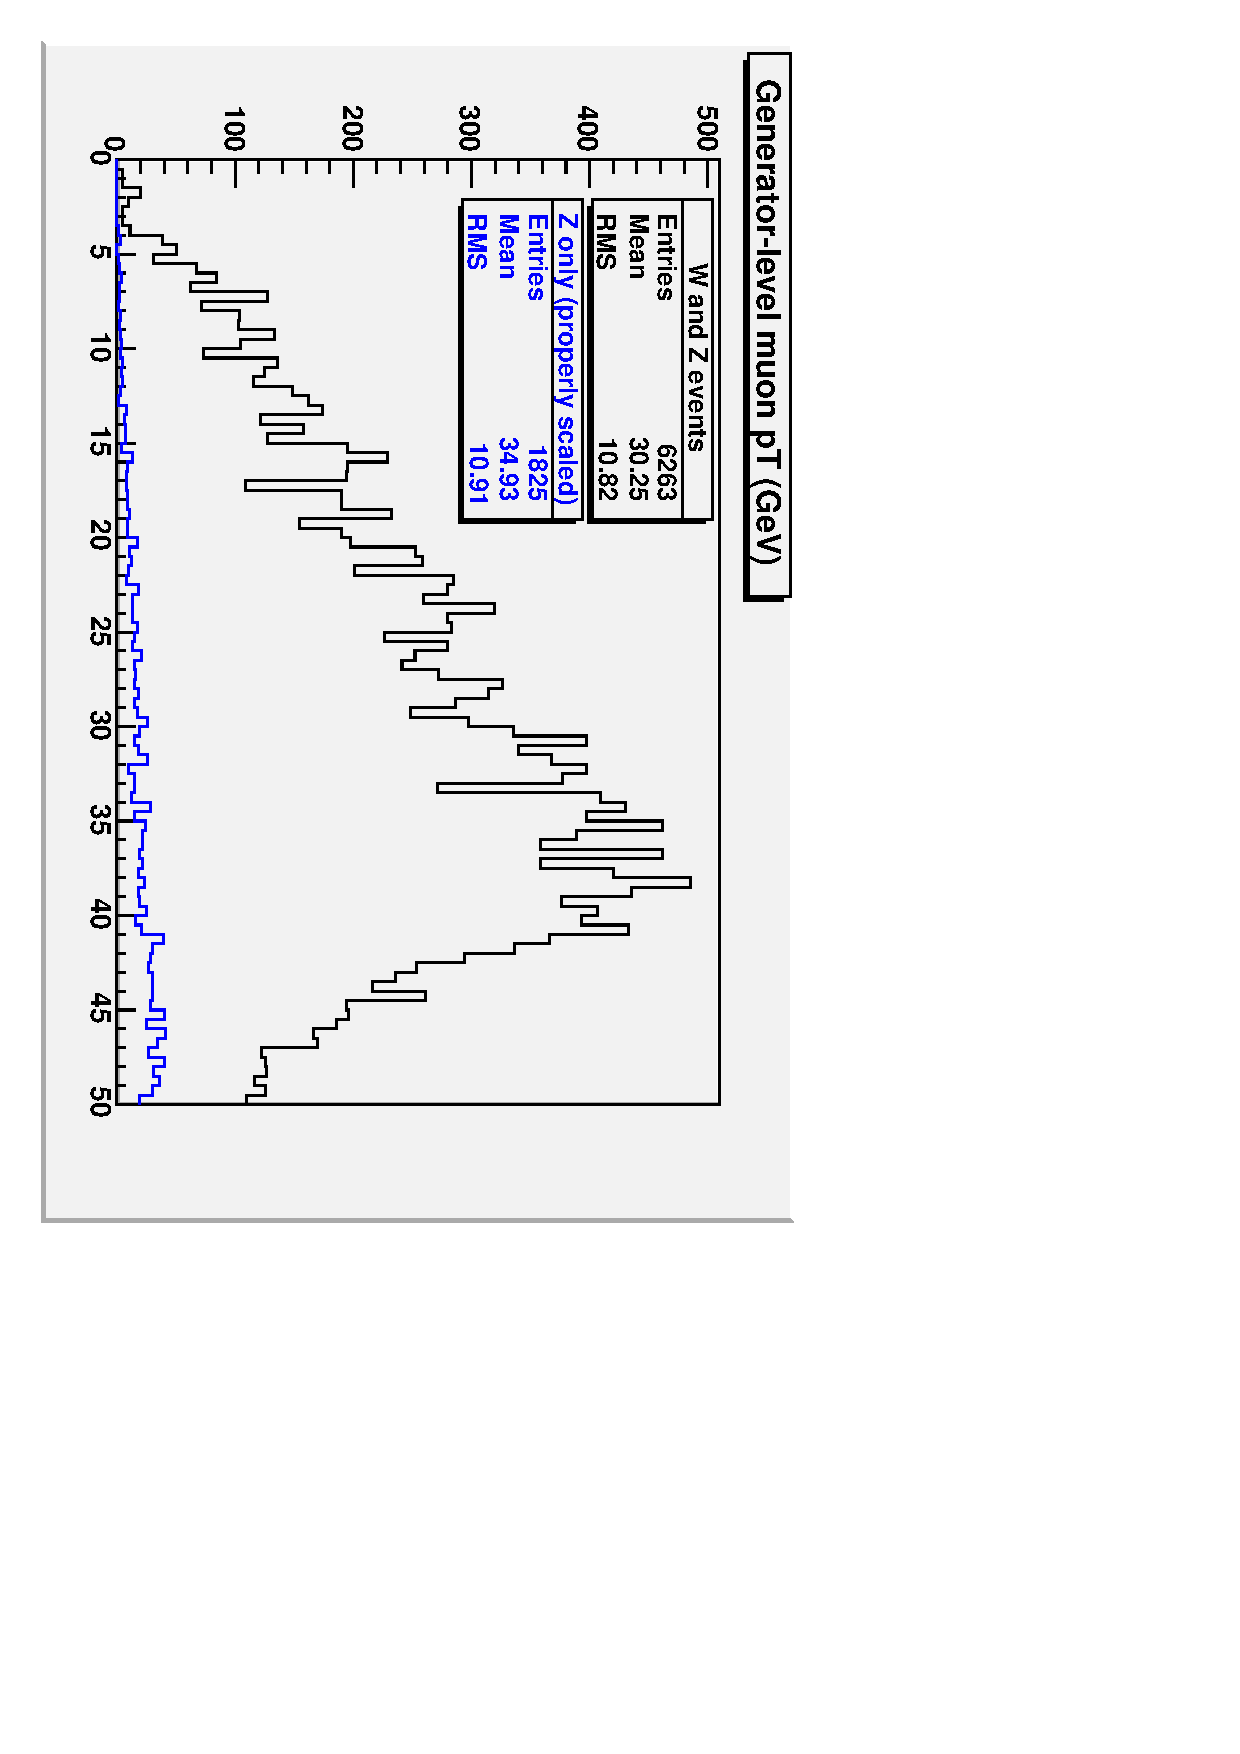
\includegraphics[height=\linewidth, angle=90]{w_and_z.pdf}
\end{frame}

\begin{frame}
\begin{center}
\begin{tabular}{c c c c}
Sample & cross-section & $k$ in $Ae^{-k \, pT}$ & $(A/k)e^{-k \, 20\mbox{\scriptsize\ GeV}}$ \\
QCD 0--30~GeV & 54.71~mb & \textcolor{blue}{0.30/GeV?} & \textcolor{blue}{0.4520?} \\
QCD 30--50~GeV & 0.1553~mb & 0.25/GeV & 0.0042 \\
QCD 50--80~GeV & 0.0216~mb & 0.17/GeV & 0.0042 \\
QCD 80~GeV--$\infty$ & 0.0037~mb & 0.11/GeV & 0.0037 \\
\end{tabular}
\end{center}

\begin{columns}
\column{0.5\linewidth}
\begin{center}
30--50~GeV: 0.46\% have muons

50--80~GeV: 1.1\% have muons

80~GeV--$\infty$: 2\% have muons
\end{center}
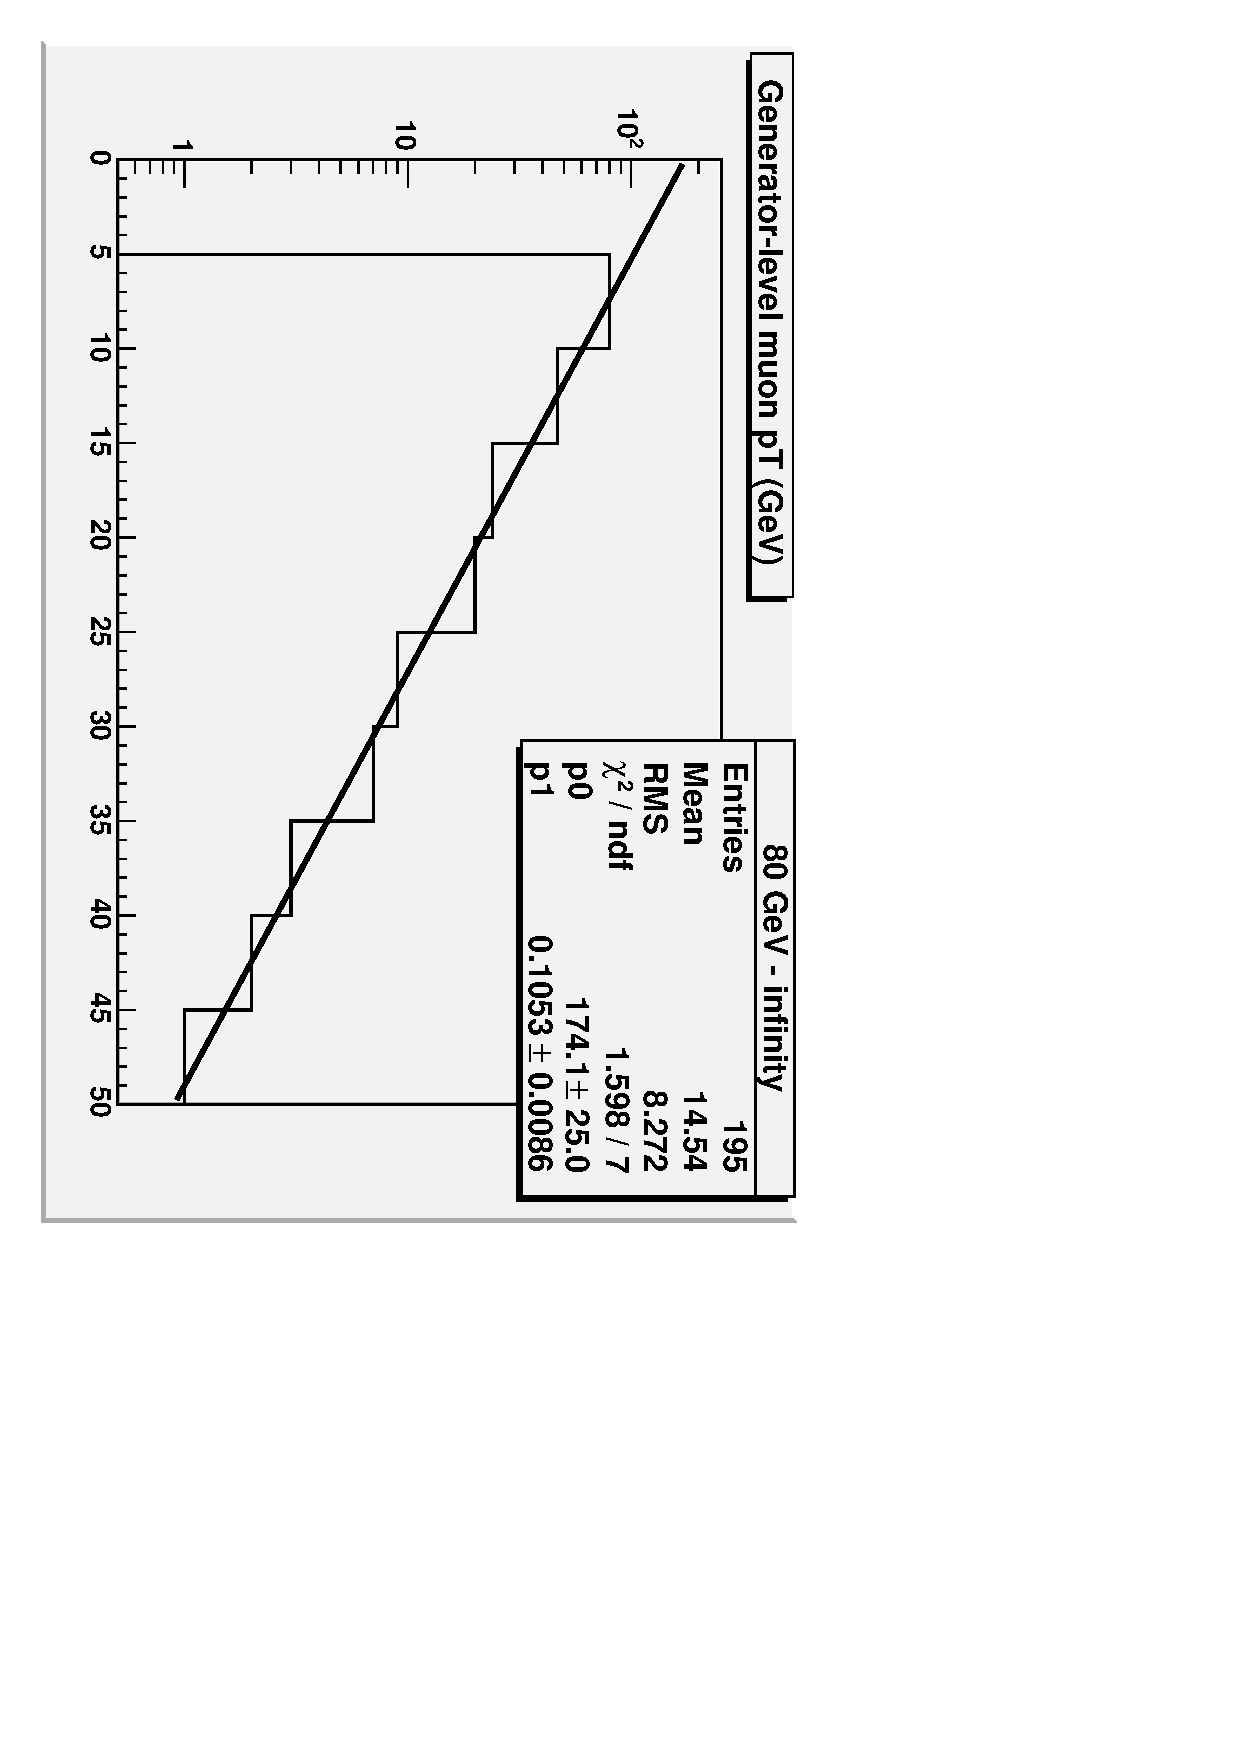
\includegraphics[height=\linewidth, angle=90]{exponential_qcd2.pdf}

\column{0.5\linewidth}
0--30~GeV: $<$ 0.01\% have muons. \\ Forget about that.

\begin{center}
Fraction with $p_T$ $>$ 20~GeV
\begin{tabular}{c c}
QCD 30--50~GeV & 3\% \\
QCD 50--80~GeV & 9\% \\
QCD 80~GeV--$\infty$ & 21\% \\
\end{tabular}
\end{center}

$\displaystyle \frac{\sigma_{\mbox{\scriptsize QCD} \mu}}{\sigma_{\mbox{\scriptsize ``physics''} \mu}} = \frac{0.000058 \mbox{ mb}}{7.1 \mbox{ nb}} = 8.2$

\end{columns}
\end{frame}

\begin{frame}
\frametitle{Do that out more explicitly, for the record}

$\displaystyle \frac{\sigma_{\mbox{\scriptsize QCD} \mu}}{\sigma_{\mbox{\scriptsize ``physics''} \mu}} = (0.1553\mbox{ mb} \cdot 0.0046 \cdot 0.03 + 0.0216\mbox{ mb} \cdot 0.011 \cdot 0.09 + 0.0037\mbox{ mb} \cdot 0.02 \cdot 0.21) / (7.1\mbox{ nb}) = \frac{0.000058 \mbox{ mb}}{7.1 \mbox{ nb}} = 8.2$

\vfill
where each term in the numerator has three factors:
\begin{itemize}
\item cross-section of the QCD process
\item fraction with $p_T$ $>$ 6~GeV muons
\item $\displaystyle \frac{\int_{20\mbox{\tiny\ GeV}}^\infty e^{-k p_T} \, dp_T}{\int_{6\mbox{\tiny\ GeV}}^\infty e^{-k p_T} \, dp_T}$
\end{itemize}


\end{frame}

\begin{frame}
\begin{itemize}
\item 100k ``physics'' muon events is 25~pb$^{-1}$ and quite enough for a good alignment (2.5~pb$^{-1}$ is barely enough).
\item To get the same muons from a realistic soup with a 20~GeV cut, anticipate $(8.2 + 1)$ times as many = 1 million
\item 17kB per muon $\to$ 16GB?  That's not very large.
\item If we try to go down to a $p_T$ $>$ 10~GeV cut (redo all math), we find QCD sample is 61 $\times$ the ``physics'' sample $\to$ 6.1 million $\to$ 100GB\ldots that's something.
\end{itemize}

\begin{center}
\begin{tabular}{c c c c}
cut & events & disk space & alignment time/iteration \\\hline
10 GeV & 6.1 million & 100 GB & 76.3 hours \\
\textcolor{blue}{15 GeV} & \textcolor{blue}{2.3 million} & \textcolor{blue}{37 GB} & \textcolor{blue}{28.7 hours} \\
20 GeV & 0.94 million & 16 GB & 11.8 hours \\
\textcolor{blue}{25 GeV} & \textcolor{blue}{0.45 million} & \textcolor{blue}{7.3 GB} & \textcolor{blue}{5.6 hours} \\
30 GeV & 0.25 million & 4.0 GB & 3.1 hours \\
\textcolor{blue}{35 GeV} & \textcolor{blue}{0.17 million} & \textcolor{blue}{2.8 GB} & \textcolor{blue}{2.1 hours} \\
40 GeV & 0.14 million & 2.3 GB & 1.8 hours \\
\end{tabular}
\end{center}
\end{frame}

\begin{frame}
We want realistic soups of the 15~GeV cut, 25~GeV, and 35~GeV.  This
will cost 50~GB.  We want the following features:
\begin{itemize}
\item Statistically independent samples: {\it different} events
\item Miscalibrated chambers (doesn't hurt: bring it on!)
\item Realistically misaligned tracker (only ONE times the short-term scenario, or the 10~pb$^{-1}$ sample, whichever is most appropriate)
\item Wheels/disks misaligned 3~mm and 1~mrad in all directions/angles
\item Chambers misaligned 3~mm and 1~mrad in all directions/angles
\item CSC layers misaligned 191~$\mu$m in $x$, 335~$\mu$m in $y$ and 0.04~mrad in $\phi_z$
\item No DT layer/superlayer misalignment
\end{itemize}
The events can come from the ``QCDmu\_Pt\_30\_50'', ``QCDmu\_Pt\_50\_80'', ``QCDmu\_Pt\_80\_120'', ``QCDmu\_Pt\_120\_170'', ``QCDmu\_Pt\_170\_230'' GEN-SIM samples.
\end{frame}

\begin{frame}
\frametitle{What will we do with them?}
\begin{itemize}
\item Wheel/disk alignment in each of the three samples with a few thousand global muons: well under an hour.
\item Global muon alignment on each sample (with deweighting).  1 iteration = 28.7 hours, 5.6 hours, 2.1 hours in parallel.  Actually, break each of these samples into three parts: 90\%, 9\%, and 1\% of the events, so you have 9 globalmuon jobs.
\item Standalone muon alignment on 1/10th of the 15~GeV cut, half of the 25~GeV cut, all of the 35~GeV cut (NO deweighting).  7 iterations = 20.1 hours, 19.6 hours, 14.7 hours in parallel.  Do the 90\%/9\%/1\% thing, so you have 9 standalonemuon jobs running.
\item Global muon alignment of layers with the three samples in parallel: 28.7 hours, 5.6 hours, 2.1 hours {\it after} the chamber alignment is done.  90\%/9\%/1\% makes for 9 layer jobs.  The clock is now at 2.5 days and we have been using 18 CPUs.
\item When they are done, re-reconstruct $N$ events in each of the 27 conditions.  NO APEs!!!
\end{itemize}

\end{frame}


\end{document}
